%  The "autowc" option automatically inserts a word count 
%  on the title page, using texcount. (The "Frontmatter" 
%  on the title page and reference list are omitted.)
%  NOTE THAT THIS WILL ONLY WORK IF YOU HAVE  
%  INSTALLED TEXCOUNT, AND HAVE ENABLED --shell-escape
%  OR --enable-write18. (These will work on Overleaf.)
%  If you get an error about "texcount not found", delete
%  the autowc option, and manually specify the wordcount 
%  with \totalwordcount{xxx}.
% autowc may cause longer compilation time. You can 
% disable it first while actively editing, and only
% enable it when you're ready to take stock and check
% on your work.
\documentclass[autowc]{CUP-JNL-PPS}

% Use these lines if you want to provide a manual word count or if you're not using texcount.
% \documentclass{CUP-JNL-PPS}
% \totalwordcount{500}

%%%% Packages
\usepackage{latexsym}
\usepackage{graphicx}
\usepackage{multicol,multirow}
\usepackage{amsmath,amssymb,amsfonts}
\usepackage{mathrsfs}
\usepackage{amsthm}
\usepackage{rotating}
\usepackage{appendix}
\usepackage[authordate16, backend=biber]{biblatex-chicago}
\addbibresource{ref.bib}
\DeclareFieldFormat{doi}{%
  doi\addcolon\space
  \ifhyperref
    {\href{https://doi.org/#1}{\nolinkurl{#1}}}
    {\nolinkurl{#1}}}
\usepackage{ifpdf}
\usepackage[T1]{fontenc}
\usepackage[type1,lining]{ebgaramond}
\usepackage[type1,lining]{sourcesanspro}
\usepackage{newtxmath}
\usepackage{textcomp}%
\usepackage{xcolor}%
\usepackage{hyperref}
\usepackage{lipsum}
%%%%

%\articletype{RESEARCH ARTICLE}
\jname{Title Pending}
%\artid{20}
\jyear{2025}
% \jvol{4}
% \jissue{1}
% \jdoi{10.1017/pps.2021.xx}
\jdoi{}
%\raggedbottom

%\usepackage{showframe}


\begin{document}

%% When using autowc (automatic wordcount, you can use %TC:ignore and %TC:endignore blocks to mark regions of text that should be omitted from counting.)
%TC:ignore
\begin{Frontmatter}
\title[Underrepresentation Theory]{
Underrepresentation Theory: Examining the approach of data collection and analysis on underrepresented people in mathematics
\thanks{
    Author N. \authororcid{0000-0002-8514-4315} Professor of Political Science at Princeton University.
    Her research targets the intersection of politics and belonging in relation to immigrant integration issues and national identity, from the point of view of minorities and majorities alike.
}
}

\author{Jillian Alexander \authororcid{0009-0001-3843-9479}, Howard University, United States}
\author{Aden Mobley, Morehouse College, United States}
\author{Sona Tau Estrada Rivera \authororcid{0009-0000-6779-8166}, Universidad de Puerto Rico, Recinto de R\'{i}o Piedras, San Juan, Puerto Rico}

\abstract{
Abstracts should be 250 words.
It must be able to stand alone and so cannot contain citations to the paper's references, equations, etc.
An abstract must consist of a single paragraph and be concise.
Because of online formatting, abstracts must appear as plain as possible.
}

\end{Frontmatter}
%TC:endignore

\onecolumn{}

\section{Introduction}

\dropcap{A}n underrepresented community is a subgroup of a larger population that all share one or more characteristics.
Given the current social landscape, underrepresented communities constantly face systemic challenges, oppression and individual power struggles.
By studying underrepresented communities, we can highlight some of the systemic challenges that they face.
However, in some cases, it is actually possible to not be able to study an underrepresented community because of a lack of data.
These systemic challenges have promoted an environment that makes it difficult to study these communities.
This brings us to our research question,
\begin{quote}
    What questions surrounding underrepresented communities in Mathematics are currently hard to answer?
\end{quote}

Many underrepresented communities participate in Mathematics.
We will focus on,
\begin{itemize}
    \item LGBTQ+ people
    \item People of colour
    \item Women
    \item Indigenous people
\end{itemize}

Research focus: Underrepresented communities in Mathematics.

\section{Datasets}
\section{Literature}
\section{Surveys}

% \begin{figure}[t]%
% \FIG{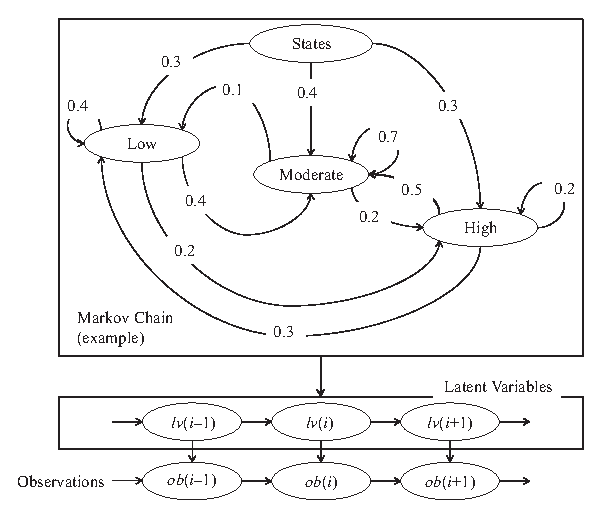
\includegraphics[width=.75\columnwidth]{Fig}}
% {\caption{This is an example of caption this is an example of caption  this is an example of caption this is an example of caption}
% \label{fig1}}
% \end{figure}

% \begin{table}[t]
%     \tabcolsep=0pt%
%     \TBL{
%         \caption{Tables which are too long to fit, should be written using the ``table*'' environment\label{tab2}}
%     }{
%         \begin{fntable}
%             \begin{tabular*}{\textwidth}{@{\extracolsep{\fill}}lcccccc@{}}
%                 \toprule%
%                 & \multicolumn{3}{@{}c@{}}{\TCH{Element 1}}& \multicolumn{3}{@{}c@{}}{\TCH{Element 2\smash{\footnotemark[1]}}} \\
%                 \cmidrule{2-4}\cmidrule{5-7}%
%                 \TCH{Project} & \TCH{Energy} & \TCH{$\boldsymbol{\sigma_{\text{calc}}}$} & \TCH{$\boldsymbol{\sigma_{\text{expt}}}$} &
%                 \TCH{Energy} & \TCH{$\boldsymbol{\sigma_{\text{calc}}}$} & \TCH{$\boldsymbol{\sigma_{\text{expt}}}$} \\
%                 \midrule
%                 \TCH{Stage 3}&990 A &168 &47$\pm$12 &78 A &66 &39$\pm$10\\
%                 {\TCH{Stage 4}}&500 A &961 &22$\pm$10 &90 A &68 &92$\pm$40\\
%                 \botrule
%             \end{tabular*}%
%             \footnotetext[]{
%                 {Note:} This is an example of table footnote this is an example of table footnote this is an example of table footnote this is an example of~table footnote this is an example of table footnote
%             }
%             \footnotetext[1]{This is an example of table footnote}%
%         \end{fntable}
%     }
%     \vspace*{7pt}
% \end{table}



% \section{Acknowledgments}
% We are grateful for the technical assistance of A. Author.


% \section{Funding Statement}
% This research was supported by grants from the <funder-name> <doi> (<award ID>); <funder-name> <doi> (<award ID>).
%%

% \begin{appendix}\appheader
% \section{Appendix. Title for Appendix Section}\label{appendixA}
% Appendix text here.
% \end{appendix}

% \theendnotes

\begin{Backmatter}

%%%\paragraph{Competing Interests}
%%%A statement about any financial, professional, contractual or personal relationships or situations that could be perceived to impact the presentation of the work --- or `None' if none exist
%%%
%%%\paragraph{Data Availability Statement}
%%%A statement about how to access data, code and other materials allowing users to understand, verify and replicate findings --- e.g. Replication data and code can be found in Harvard Dataverse: \verb+\url{https://doi.org/link}+.
%%%
%%%\paragraph{Ethical Standards}
%%%The research meets all ethical guidelines, including adherence to the legal requirements of the study country.
%%%
%%%\paragraph{Author Contributions}
%%%Please provide an author contributions statement using the CRediT taxonomy roles as a guide {\verb+\url{https://www.casrai.org/credit.html}+}. Conceptualization: A.A; A.B. Methodology: A.A; A.B. Data curation: A.C. Data visualisation: A.C. Writing original draft: A.A; A.B. All authors approved the final submitted draft.
%%%
%%%\paragraph{Supplementary Material}
%%%State whether any supplementary material intended for publication has been provided with the submission.

\printbibliography

\end{Backmatter}


\end{document}
